\chapter{Lecture 5: Building a Black Hole and the Near-Horizon Puzzle}

These notes follow Leonard Susskind's fifth supplementary lecture in \emph{Cosmology and Black Holes} and are curated by LazyingArt LLC. The lecture begins lightly, with a rough estimate of a black hole whose temperature matches the \(3\,\mathrm{K}\) cosmic microwave background, but that estimate is only a warm-up. The real task is then stated very plainly: build a black hole, not by solving the full Einstein equations in detail, but by assembling a few geometric ingredients, reading the basic mathematics from Penrose diagrams, and only afterward turning to the thermodynamic and quantum puzzles near the horizon.

\section{Warm-Up: A Three-Degree Black Hole}

The opening question is deliberately informal: what mass would a black hole have if its Hawking temperature were of order \(3\,\mathrm{K}\)? The motivation is that the microwave background sets the temperature scale of otherwise empty space, so a \(3\,\mathrm{K}\) black hole would, very roughly, be in equilibrium with its surroundings. Susskind immediately notes that this equilibrium would be unstable, but he keeps the estimate as a scale-setting exercise.

The estimate is of the simplest kind. Radiation at a few kelvin has wavelength in the microwave range, and in the lecture Susskind takes that wavelength to be of order centimeters. His heuristic is then that the typical wavelength emitted by a black hole is of the same order as the black-hole radius. Thus
\begin{equation}
R_s \sim \lambda_{\text{thermal}} \sim 1\,\mathrm{cm}.
\end{equation}
Once the radius is known, the mass follows from the Schwarzschild relation
\begin{equation}
R_s=\frac{2GM}{c^2}.
\end{equation}
A solar-mass black hole has radius of order kilometers, so a black hole of radius \(1\,\mathrm{cm}\) is smaller in radius by roughly \(10^5\), and therefore smaller in mass by the same factor:
\begin{equation}
\frac{M}{M_\odot}\sim \frac{R_s}{R_{s,\odot}}\sim 10^{-5}.
\end{equation}
This puts the answer in the planetary range. Susskind calls it roughly Earth mass; a student reports a value closer to Moon mass. The lecture is clear that this is only an order-of-magnitude estimate, and it should be read that way.

At that point he cuts off the numerical discussion: let us not get lost in it; we want to build ourselves a black hole. That sentence sets the method for the rest of the lecture. The calculation is too hard. The pictures will do the work.

\section{The Two Working Parts: Flat Space and Schwarzschild}

Susskind next identifies the first two ``working parts'' of the construction: the Penrose diagram for flat space and the Penrose diagram for the Schwarzschild black hole. The lecture slows down here, but for a good reason. These are not textbook recaps inserted for completeness; they are the pieces that will shortly be sewn together.

\subsection{Flat Space in Reduced \((t,r)\) Coordinates}

The flat-space picture is drawn in reduced coordinates \((t,r)\), with the angular variables suppressed. Radial distance never goes negative, so one keeps only the half-plane \(r\geq 0\). Every point in the reduced diagram really stands for a two-sphere of angles.

Radial null rays move at \(45^\circ\): incoming light runs down and toward the origin, outgoing light runs up and away from it. The Penrose diagram is then obtained by a conformal compactification of this half-plane. Susskind calls the procedure ``smushing,'' and the joke is useful because it captures exactly the visual point: an infinite region is compressed into a finite wedge, while the null directions remain at \(45^\circ\).

\begin{figure}[ht]
\centering

\includegraphics[width=0.62\textwidth]{lecture_05_figure_02.png}
\caption{Upper half of the compactified flat-space Penrose diagram on the board. At this moment in the lecture Susskind deliberately leaves the lower half undrawn.}
\end{figure}

The board image is valuable evidence here. It shows the left timelike boundary, the sharp right tip, the top label \(t=\infty\), and the two families of compressed curves. It also shows the choice Susskind makes in the lecture: he draws only the upper half, because that is all he needs for the causal story he is telling at that moment.

\begin{figure}[ht]
\centering
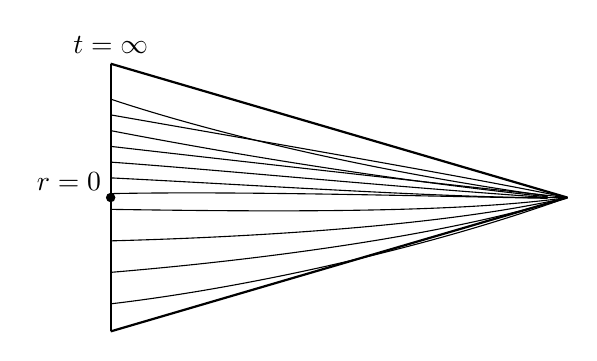
\begin{tikzpicture}[scale=1.0]
\draw[thick] (0,0) -- (0,3.4);
\draw[thick] (0,3.4) -- (5.8,1.7);
\draw[thick] (0,0) -- (5.8,1.7);

\fill (0,1.7) circle (0.06);

\draw (0,0.35) .. controls (1.7,0.55) and (4.0,1.05) .. (5.8,1.7);
\draw (0,0.75) .. controls (1.8,0.90) and (4.2,1.20) .. (5.8,1.7);
\draw (0,1.15) .. controls (1.9,1.20) and (4.3,1.35) .. (5.8,1.7);
\draw (0,1.55) .. controls (2.0,1.52) and (4.4,1.50) .. (5.8,1.7);
\draw (0,1.95) .. controls (2.0,1.85) and (4.5,1.68) .. (5.8,1.7);
\draw (0,2.35) .. controls (2.0,2.12) and (4.6,1.83) .. (5.8,1.7);
\draw (0,2.75) .. controls (2.0,2.40) and (4.6,1.95) .. (5.8,1.7);

\draw (0,2.95) .. controls (1.2,2.55) and (3.2,2.05) .. (5.55,1.72);
\draw (0,2.55) .. controls (1.3,2.30) and (3.3,1.95) .. (5.55,1.71);
\draw (0,2.15) .. controls (1.4,2.05) and (3.4,1.85) .. (5.55,1.70);
\draw (0,1.75) .. controls (1.5,1.78) and (3.5,1.73) .. (5.55,1.69);

\node[left] at (0,1.9) {$r=0$};
\node[above] at (0,3.4) {$t=\infty$};
\end{tikzpicture}
\caption{Cleaned reconstruction of the upper half of the compactified flat-space diagram. The curve shapes are qualitative; what matters is the crowding of the constant-\(r\) and constant-\(t\) families near infinity.}
\end{figure}

The lecture makes several concrete points from this diagram. First, lines of constant \(r\), vertical in the unsquashed picture, become bowed curves that accumulate toward the compactified infinity. Second, lines of constant \(t\) do the same as one approaches the top of the wedge. Third, one should read the diagram operationally, not just topologically: a light ray emitted from the origin goes out at \(45^\circ\), a light ray sent in from far away comes in at \(45^\circ\), and a light ray that misses the origin by some finite impact parameter still looks, when far away, very much like a radial ray. Only near its point of closest approach does it reveal that it does not actually hit \(r=0\).

This completes the first working part. It is not yet a black hole; it is the causal geometry of ordinary empty spacetime written in the reduced \((t,r)\) language that will later let the black hole be constructed.

\subsection{The Schwarzschild Penrose Diagram}

The second working part is the Penrose diagram of the eternal Schwarzschild solution. Susskind redraws it from scratch: a diamond, then a second diamond beside it, then wavy lines across the top and bottom. Those wavy lines represent the future and past singularities. He immediately warns that one of the exteriors is not going to matter for the construction to come; the full eternal diagram contains more structure than a black hole formed by collapse will actually need.

\begin{figure}[ht]
\centering

\includegraphics[width=0.72\textwidth]{lecture_05_figure_03.png}
\caption{Schwarzschild Penrose diagram on the board, with representative constant-\(r\) and constant-time curves in the right exterior region.}
\end{figure}

In the board image the right-hand exterior diamond is the useful one. Its right tip is labeled \(r=\infty\), its upper and lower vertices are labeled \(t=\infty\) and \(t=-\infty\), and the family of hand-drawn interior curves is being used to read the Schwarzschild coordinates. The singularity labels are only partially legible on the board, so the notes standardize them as future and past singularity.

\begin{figure}[ht]
\centering
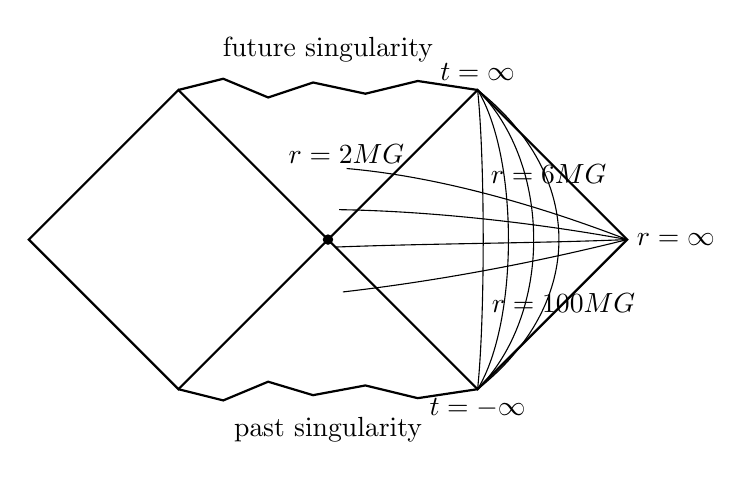
\begin{tikzpicture}[scale=0.95]
\coordinate (C) at (0,0);
\coordinate (LT) at (-2,2);
\coordinate (LL) at (-4,0);
\coordinate (LB) at (-2,-2);
\coordinate (RT) at (2,2);
\coordinate (RR) at (4,0);
\coordinate (RB) at (2,-2);

\draw[thick] (C) -- (LT) -- (LL) -- (LB) -- (C);
\draw[thick] (C) -- (RT) -- (RR) -- (RB) -- (C);

\draw[thick] (-2,2) -- (-1.4,2.15) -- (-0.8,1.9) -- (-0.2,2.1) -- (0.5,1.95) -- (1.2,2.12) -- (2,2);
\draw[thick] (-2,-2) -- (-1.4,-2.15) -- (-0.8,-1.9) -- (-0.2,-2.08) -- (0.5,-1.95) -- (1.2,-2.12) -- (2,-2);

\fill (C) circle (0.07);

\draw (2,2) .. controls (2.10,1.05) and (2.10,-1.05) .. (2,-2);
\draw (2,2) .. controls (2.55,1.10) and (2.55,-1.10) .. (2,-2);
\draw (2,2) .. controls (3.00,1.00) and (3.00,-1.00) .. (2,-2);
\draw (2,2) .. controls (3.45,0.85) and (3.45,-0.85) .. (2,-2);

\draw (0.25,0.95) .. controls (1.4,0.85) and (2.7,0.50) .. (4,0);
\draw (0.15,0.40) .. controls (1.4,0.38) and (2.8,0.22) .. (4,0);
\draw (0.10,-0.10) .. controls (1.4,-0.05) and (2.8,-0.05) .. (4,0);
\draw (0.20,-0.70) .. controls (1.5,-0.55) and (2.8,-0.30) .. (4,0);

\node[above] at (2,2) {$t=\infty$};
\node[below] at (2,-2) {$t=-\infty$};
\node[right] at (4,0) {$r=\infty$};
\node[left] at (1.15,1.15) {$r=2MG$};
\node at (2.95,0.88) {$r=6MG$};
\node at (3.15,-0.85) {$r=100MG$};
\node[above] at (0.0,2.25) {future singularity};
\node[below] at (0.0,-2.25) {past singularity};
\end{tikzpicture}
\caption{Cleaned reconstruction of the Schwarzschild diagram as used in the lecture. The internal grid is schematic and is intended only to show the qualitative behavior of constant-\(r\) and constant-time curves.}
\end{figure}

Several statements are read directly from this picture. Far from the black hole, the right exterior looks much like the compactified flat-space wedge. The horizon-side edge of that exterior corresponds to
\begin{equation}
r=2MG
\end{equation}
in the lecture's \(c=1\) shorthand, and farther out one may draw representative constant-\(r\) curves such as
\begin{equation}
r=6MG,
\qquad
r=100MG.
\end{equation}
These are not exact coordinate plots on the board; they are sample radii that show how the exterior geometry approaches the flat-space picture as one moves away from the hole.

Near the center, however, the comparison with flat space breaks down sharply. In flat space a radial light ray can reach \(r=0\) and then re-emerge. In Schwarzschild there is no such bounce. A future-directed light ray that enters the black hole crosses the horizon and runs into the singularity. That is the decisive difference. Far away the two diagrams look alike; near the hole they do not.

\section{Newton's Theorem, Birkhoff's Theorem, and the Missing Ingredient}

With the two static pictures in place, Susskind announces that one more ingredient is needed. The Penrose diagrams alone do not yet say how to create a black hole. The needed principle is Newton's shell theorem and its relativistic generalization, Birkhoff's theorem.

\paragraph{Newton's theorem.} For any spherically symmetric mass distribution, the gravitational field at a given radius depends only on the mass enclosed within that radius. Matter outside the chosen sphere contributes nothing to the net force there. In particular, for a hollow spherical shell one has
\begin{equation}
g_{\text{inside shell}}=0,
\qquad
g_{\text{outside shell}}=\frac{GM}{r^2}
\end{equation}
for a shell of total mass \(M\). Susskind emphasizes the shell case because that is the one he is about to use.

\paragraph{Birkhoff's theorem.} The relativistic statement has exactly the same logic. Inside a spherically symmetric shell the metric is just flat Minkowski spacetime. Outside the shell the metric is Schwarzschild with the shell's total mass. In the lecture this is the operational content:
\begin{equation}
\text{inside shell} \longrightarrow \text{Minkowski},
\qquad
\text{outside shell} \longrightarrow \text{Schwarzschild}(M).
\end{equation}
Two points matter. First, the theorem is not tied to a static shell; the shell may be moving, provided spherical symmetry is preserved. Second, the shell may be a shell of radiation just as well as a shell of ordinary matter. That is exactly what the next construction requires.

\section{A Black Hole from a Collapsing Shell of Light}

Susskind now turns to what he calls the simplest way of creating a black hole. One imagines a spherically symmetric shell of light collapsing inward. He motivates the picture by analogy with a perfectly symmetric arrangement of lasers, but then strips away the engineering details and keeps only the idealized shell itself.

The shell carries some total energy \(E\). From far away, one can associate to it the mass parameter
\begin{equation}
M=\frac{E}{c^2}.
\end{equation}
In the lecture Susskind immediately simplifies the notation and, in effect, works in units where energy and mass are not distinguished:
\begin{equation}
E=M.
\end{equation}
The shell moves inward at the speed of light, so on the Penrose diagram it is represented by an ingoing null line. Every point on that line is really a two-sphere, so the line is not a single light ray in space; it is a spherical shell of radiation.

\begin{figure}[ht]
\centering

\includegraphics[width=0.72\textwidth]{lecture_05_figure_05.png}
\caption{Board layout at the transition to the collapse construction. The earlier flat-space wedge remains on the left, the Schwarzschild diagram on the right, and Susskind is about to combine them.}
\end{figure}

This transition image is documentary evidence rather than a finished mathematical figure. Its value is precisely that it shows the lecture's sequencing: the flat-space Penrose diagram has been kept on the board, the Schwarzschild diagram has been kept on the board, and the next move is to sew them together.

The construction then proceeds by successive corrections to the two earlier pictures.

\begin{enumerate}
\item Begin with the Penrose diagram of empty flat space.
\item Draw an ingoing null line representing the collapsing shell of light arriving from infinity.
\item In that flat-space picture, the region below and to the left of the shell is the interior of the shell; by Birkhoff's theorem it is correctly described as flat spacetime.
\item Now take the Schwarzschild diagram and draw the corresponding ingoing null shell there.
\item In that picture, the region above and to the right of the shell is the exterior of the shell; by Birkhoff's theorem it is correctly described by the Schwarzschild metric.
\item Erase the regions that are wrong for the collapse problem: the white-hole region, the second exterior, and the interior portion of the eternal diagram that is not part of the actual collapse.
\item Match the endpoint of the collapsing shell, where it reaches \(r=0\) in the flat picture, to the endpoint where it reaches the singularity in the Schwarzschild picture.
\end{enumerate}

\begin{figure}[ht]
\centering
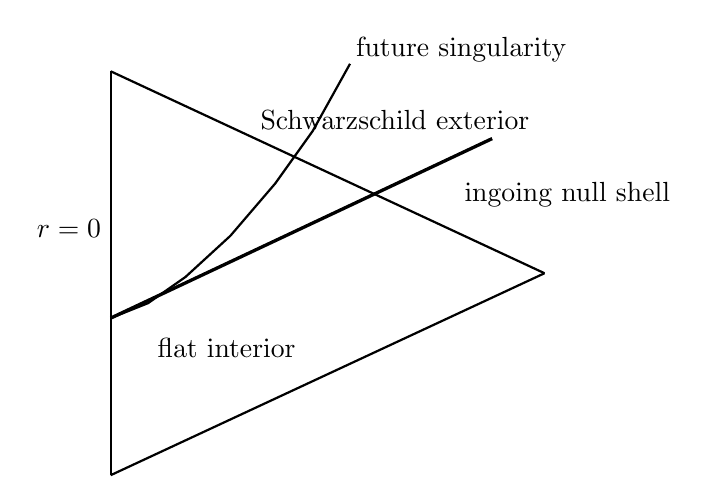
\begin{tikzpicture}[scale=0.95]
\coordinate (O) at (0,-2.3);
\coordinate (P) at (0,3.1);
\coordinate (I) at (5.8,0.4);
\coordinate (S0) at (5.1,2.2);
\coordinate (C0) at (0,-0.2);

\draw[thick] (O) -- (P);
\draw[thick] (P) -- (I);
\draw[thick] (O) -- (I);

\draw[very thick] (S0) -- (C0);

\draw[thick] (0,-0.2) -- (0.5,0.0) -- (1.0,0.35) -- (1.6,0.9) -- (2.2,1.6) -- (2.7,2.3) -- (3.2,3.2);

\node[left] at (0,1.0) {$r=0$};
\node[right] at (4.6,1.45) {ingoing null shell};
\node at (1.55,-0.6) {flat interior};
\node at (3.8,2.45) {Schwarzschild exterior};
\node[above right] at (3.15,3.1) {future singularity};
\end{tikzpicture}
\caption{Transcript-driven reconstruction of the black-hole formation diagram. The spacetime below the shell is flat, the spacetime above it is Schwarzschild, and the shell itself is the seam along which the two pieces are pasted together.}
\end{figure}

This is the simplest collapse geometry of the lecture. It explains, at a stroke, what becomes of the surplus regions of the eternal Schwarzschild diagram. There is no white hole. There is no second universe. There is, however, still a singularity, because the collapsing shell reaches \(r=0\) and the geometry above it is genuinely black-hole exterior geometry.

\section{Where the True Horizon Is}

Once the collapse geometry has been assembled, Susskind turns to the most conceptually important correction of the lecture. So far, he says, we have not even talked about the true horizon. The line \(r=2MG\) in the eternal Schwarzschild diagram was only a provisional guide. The real horizon is defined causally.

\begin{definition}
The event horizon is the boundary in spacetime between events from which an outgoing light ray can still reach infinity and events from which no outgoing light ray can escape to infinity.
\end{definition}

In the collapse diagram, the event horizon is found by drawing the outgoing null line that just barely fails to escape. Everything to one side can still send a signal out to infinity. Everything to the other side cannot.

\begin{figure}[ht]
\centering
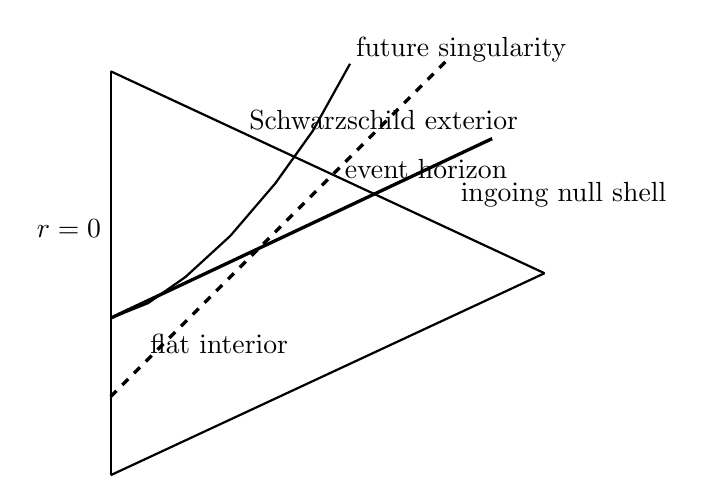
\begin{tikzpicture}[scale=0.95]
\coordinate (O) at (0,-2.3);
\coordinate (P) at (0,3.1);
\coordinate (I) at (5.8,0.4);
\coordinate (S0) at (5.1,2.2);
\coordinate (C0) at (0,-0.2);
\coordinate (H0) at (0,-1.25);

\draw[thick] (O) -- (P);
\draw[thick] (P) -- (I);
\draw[thick] (O) -- (I);

\draw[very thick] (S0) -- (C0);

\draw[thick] (0,-0.2) -- (0.5,0.0) -- (1.0,0.35) -- (1.6,0.9) -- (2.2,1.6) -- (2.7,2.3) -- (3.2,3.2);

\draw[dashed,very thick] (H0) -- (2.6,1.35) -- (4.5,3.25);

\node[left] at (0,1.0) {$r=0$};
\node[right] at (4.55,1.45) {ingoing null shell};
\node[right] at (3.0,1.8) {event horizon};
\node at (1.45,-0.55) {flat interior};
\node at (3.65,2.45) {Schwarzschild exterior};
\node[above right] at (3.15,3.1) {future singularity};
\end{tikzpicture}
\caption{Causal reconstruction of the event horizon in the collapse geometry. The dashed line begins in the flat region before the shell arrives and later becomes the usual Schwarzschild horizon.}
\end{figure}

This figure carries the main surprise of the lecture. Part of the event horizon lies in a region that is still locally flat. The shell has not yet arrived there; nothing dramatic is happening there; nevertheless it is already impossible for an event behind that boundary to send a signal to infinity. The global future of the spacetime has already decided the issue.

That is the point of the drain-hole analogy that Susskind brings in at this stage. One may be sitting in calm water, with no local flow at all, and yet already be doomed if the drain is about to be opened and the future current will be too strong to row against. The analogy is not meant to replace the Penrose-diagram argument; it is meant only to make the causal point emotionally intuitive.

The horizon is also a growing two-sphere. Every point of the reduced diagram represents an \(S^2\), so one can ask for the size of the horizon-sphere along the dashed line. At its beginning that size is zero. As one moves upward along the horizon it grows continuously, even through the flat region, until it reaches the usual Schwarzschild size
\begin{equation}
R_s=\frac{2GM}{c^2}
\end{equation}
or, in the lecture's shorthand, \(2MG\). After that it remains fixed unless additional matter falls in.

The lecture then lingers on the outside point of view. An observer at infinity can see that the black hole has formed, because the incoming shell is visible from the outside. But the same observer also describes infalling matter as collecting ever closer to the horizon. This is the beginning of the later ``plastered on the horizon'' language, and it helps explain why the next discussion of entropy proportional to horizon area feels natural in the lecture rather than artificially imposed.

\section{Horizon Entropy, Hawking Temperature, and Local Temperature}

Only after the causal structure has been made clear does Susskind pivot to what he calls the really bizarre questions: black holes, gravity, quantum mechanics, and information. He redraws the horizon in a different style, no longer as a line on a Penrose diagram but as an approximately flat surface, just as one often replaces the spherical Earth by a local flat-Earth approximation.

He begins by recalling two facts from earlier lectures. First, black holes have entropy, and that entropy is proportional to the horizon area. Second, when bits are added to the hole, the area increases in Planck-sized increments. The lecture does not re-derive the full entropy formula here; it uses the area law mainly as motivation for taking the horizon seriously as the place where information seems, from the outside, to reside.

He then recalls the Hawking temperature. In standard SI form,
\begin{equation}
T_H=\frac{\hbar c^3}{8\pi GM k_B},
\end{equation}
while in the lecture's convention, where \(k_B=1\),
\begin{equation}
T_H=\frac{\hbar c^3}{8\pi GM}.
\end{equation}
Using
\begin{equation}
R_s=\frac{2GM}{c^2},
\end{equation}
one can rewrite the temperature as
\begin{equation}
T_H=\frac{\hbar c}{4\pi R_s}
\qquad (k_B=1),
\end{equation}
so the main scaling law is
\begin{equation}
T_H\propto \frac{1}{R_s}.
\end{equation}
This is the point Susskind wants to emphasize: large black holes are cold.

At this point the lecture slows down again and asks what temperature means in a gravitational field. The question is essential because the Hawking temperature is a temperature measured far from the black hole, while the puzzle of the lecture concerns the region near the horizon. Susskind's answer is practical. A thermometer measures the kinetic energy of the particles or photons that strike it. In a gravitational field, particles that rise lose kinetic energy, and particles that fall gain it. The same is true of photons: they are redshifted as they climb and blueshifted as they fall.

He illustrates the point with a heated Earth and a very dilute atmosphere. If the ground heats molecules from below and those molecules then rise and fall in the Earth's gravitational field, a thermometer held low and a thermometer held high will not record the same local kinetic energies. Thus, for the purposes of the lecture, one should not imagine that ``thermal equilibrium in a gravitational field'' means identical local thermometer readings everywhere.

That is the bridge to the black hole. The Hawking temperature \(T_H\) is what a thermometer reads far away. One may then extrapolate inward and ask what the local temperature would be near the horizon. Susskind states the result without deriving it in detail:
\begin{equation}
T(\rho)=\frac{1}{2\pi \rho},
\end{equation}
where \(\rho\) is the proper distance from the horizon, and from this point onward in the near-horizon discussion we follow the lecture in using natural units \(c=\hbar=k_B=1\). The important feature is the divergence:
\begin{equation}
\rho\to 0
\qquad \Longrightarrow \qquad
T(\rho)\to \infty.
\end{equation}

This is the origin of the near-horizon atmosphere picture. If one lowers a tiny thermometer on a cable toward the horizon, the recorded temperature rises and rises. If one lowers an atom toward the horizon, then according to this extrapolated local temperature the environment becomes hotter and hotter. On that picture an atom should first be excited, then ionized, and, if one keeps going, ultimately torn apart. Susskind even phrases it colloquially: put your feet near the horizon and you get a hot foot.

But that is exactly where the lecture's tension appears. The horizon, viewed in the collapse geometry, was not a place of large curvature or dramatic local structure. A freely falling observer crosses it in finite proper time and, in the usual large-black-hole approximation, does not feel a special bump there. How can those two descriptions be reconciled?

\section{The Operational Argument: Heisenberg Near the Horizon}

Susskind's answer is not to settle the question by declaration. Instead, he reformulates it operationally. Can one design an experiment that decides whether an atom falling toward the horizon was or was not heated and ionized before it crossed?

He sharpens the tension using hydrogen. The relevant ionization scale is of order \(13.6\,\mathrm{eV}\); in the lecture this is discussed loosely as a temperature of a few thousand degrees. The precise numerical conversion is not the point. The point is that there is some proper distance \(\rho\) above the horizon at which the extrapolated local temperature reaches the ionization scale. If the hot-atmosphere picture is taken literally, the atom should be ionized already there, still outside the horizon, and should in principle be able to send information outward. But from the freely falling point of view the atom should be able to say: nothing special is happening to me.

At this point Susskind explicitly invokes Heisenberg. The relevant logic is the standard one. If one wants to determine the position of a particle to within a spatial resolution \(\Delta x\), one needs probing radiation with wavelength no larger than \(\Delta x\):
\begin{equation}
\lambda \lesssim \Delta x.
\end{equation}
That in turn implies a photon momentum of order
\begin{equation}
p_\gamma \gtrsim \frac{\hbar}{\Delta x}.
\end{equation}
The photon kicks the particle, and the act of measurement creates the very momentum disturbance that the experiment was designed to rule out. The conclusion is not a philosophical slogan; it is an energy-and-resolution estimate.

Now apply the same reasoning to the falling atom. Let \(\rho\) denote the proper distance from the horizon at which the local temperature first reaches the ionization scale. By the time the atom reaches that layer it is falling inward at nearly the speed of light, so the remaining proper time before it crosses the horizon is only
\begin{equation}
\Delta t \sim \frac{\rho}{c}.
\end{equation}
Once the atom is across the horizon, no information can be recovered. Therefore the experiment must determine the atom's state during this short interval while it is still outside.

But to do that, the atom must be resolved over a spatial scale of order \(\rho\). That means the probing radiation must satisfy
\begin{equation}
\lambda \lesssim \rho.
\end{equation}
Since \(E_\gamma=p_\gamma c\), the probe energy must therefore obey
\begin{equation}
E_\gamma \gtrsim \frac{\hbar c}{\rho}.
\end{equation}
In natural units this is exactly the same scale as the local temperature:
\begin{equation}
E_\gamma \sim \frac{1}{\rho}\sim T(\rho).
\end{equation}
So the experiment is trapped in a catch-22. In order to determine whether the atom has already been ionized by the near-horizon environment, one must hit it with quanta energetic enough to ionize it. The measurement does not gently inspect the atom; it supplies precisely the kind of energy that the hot-atmosphere picture attributes to the environment.

Susskind broadens the point immediately. One might imagine not shining an external photon on the atom, but instead having the atom or a nearby laboratory emit the signal outward. That does not help. The quanta carrying that signal must still have the necessary energy in the near-horizon region in order to escape and convey the information. They may later redshift as they climb out, but the atom itself only cares about the energy with which it was struck, or the energy with which it emitted the signal, in the local region near the horizon.

The same logic applies to a thermometer dropped freely toward the horizon. One cannot ``just ask the thermometer later'' without some exchange of quanta. Any information that returns to the outside must come back in the form of radiation emitted or scattered by the object, and the needed quanta again carry exactly the energy scale that the near-horizon thermal atmosphere would have carried.

This yields the limited conclusion of the lecture. One has \emph{not} proved that the infalling atom definitely feels nothing, nor has one proved that it definitely burns up in any absolute observer-independent sense. What has been shown is subtler and more operational:
\begin{equation}
\text{no external experiment can confirm ``the atom was not heated'' without itself causing heating or ionization.}
\end{equation}
That is why Susskind refuses to overstate the result. If an experiment is performed, the experiment creates the very condition it was meant to disprove. If no experiment is performed, then, at the end of the lecture, he is unwilling to assign a stronger operational meaning to the question. He explicitly compares the situation to the two-slit experiment: without the measurement, the more detailed question is not one the present analysis can answer.

\section{Summary}

The lecture unfolds in three distinct stages. It begins with a rough estimate of a \(3\,\mathrm{K}\) black hole, only to set the scale. It then turns to the actual construction of a black hole from pictures: the compactified \((t,r)\) diagram of flat space, the exterior region of the Schwarzschild Penrose diagram, and the Newton--Birkhoff shell logic that allows those two geometries to be pasted together along a collapsing null shell. That construction reveals the true event horizon as a causal boundary and shows the most striking classical fact of the lecture: the horizon forms before the shell reaches some regions, even though those regions are still locally flat.

Only then does the lecture pivot to thermodynamics. From far away one measures the Hawking temperature \(T_H\), small for a large black hole; extrapolated toward the horizon, one finds the local temperature \(T(\rho)=1/(2\pi\rho)\), which becomes large as \(\rho\to 0\). The closing Heisenberg-style argument does not resolve the horizon puzzle by ontology. It resolves it operationally: any experiment capable of checking whether an atom did or did not heat up near the horizon necessarily injects quanta of exactly the energy needed to produce that heating. That is the precise limit the lecture establishes, and it is the right place to stop.